\documentclass{article}

\usepackage{CJKutf8}
\usepackage{multicol}
\usepackage[margin=0.5cm]{geometry}
\usepackage{listings}
\usepackage{graphicx}
\graphicspath{ {./img/} }

\title{\textbf{\LARGE {HW2 Branch Predictor Design}}}
\author{學號:0711282 邱頎霖}
\date{}

\begin{document}
\begin{CJK*}{UTF8}{bsmi}
\setlength{\columnsep}{1cm}

\vspace*{-50pt}
    {\let\newpage\relax\maketitle}

\begin{multicols}{2}

\begin{center}
    \section*{INTRODUCTION}
\end{center}

\begin{flushleft}
    \ \ \ \ \ \ 在使用老師所提供的 \ string.c 所得到的\ DMIPS 為\ 0.90342 以此作為初始基準值, \
    此篇報告首先討論分支預測的必要性, 透過將分支預測給關閉可以發現\ DMIPS 下降到\ 0.87832。\
    接著討論\ BHT table entry size 對 \ DMIPS 的影響,\
    並實際將\ BHT entry 從\ 32 改到\ 64 可以獲得 DMIPS 0.97457, \
    將\ size 縮小時可以發現對 \ DMIPS 不影響仍為\ 0.90342,\
    透過\ ILA 可以發現原因是\ Dhrystone 內的迴圈總共含有\ 36 條\ branch instruction。\
    接著討論當前 Aquila 實現分支預測的方式與其缺點與分支預測的必要性,\
    並說明\ Two-level Branch Predictor 可以解決當前缺點的原因,\
    並透過以組合語言改寫得到新的\ benchmark,\
    再將當前\ Aquila 的分支預測器與\ Two-level Branch Predictor 分別都執行新的\ benchmark,\
    得到\ Two-level Branch Predictor 所花費時間少於當前\ Aquila 的結果,\
    最後以\ Dhrystone 對改寫的\ Two-level Branch Predictor 測試獲得的\ DMIPS 為\ 0.94859。
\end{flushleft}

\begin{center}
    \section*{ANALYZE}
\end{center}

\begin{flushleft}
    \ \ \ \ \ \ 根據 Aquila 的原始碼,可以知道在\ Aquila 中的分支預測為\ Dynamic branch prediction,\
    以\ 2-bit saturating counter 紀錄\ state machine 狀態且根據預測成功與失敗改變 \ state machine 狀態, \
    原始 Aquila 中以\ 32 個欄位的\ BHT 紀錄\ branch 指令與其狀態機狀態,\
    我的想法是先嘗試改變\ BHT 的大小觀察 \ DMIPS 是否上升。\newline
    
    \ \ \ \ \ \ 先考慮在沒有分支預測的情況,\
    勢必要到\ pipeline stage 中的 \ execute stage 才可以知道分支結果,\
    一旦需要跳到其他指令處非往下執行就需要做 \ flush,\
    因此即便所有分支預測都錯誤也不過會變成與不使用分支預測一樣的結果,\
    但是一旦預測成功一次便可以省下兩個 \ cycle,\
    因此確認分支預測一定是有好處的。\newline

    \ \ \ \ \ \ 接著考慮 \ BHT 大小對分支預測的影響, 一旦出現不在 \ BHT 的指令,\
    我們就得犧牲掉 \ BHT 中一條指令, 接著將新指令的狀態機初始化並將其\ PC 作為\ index 加入 \ BHT 中,\
    第一個需要注意的地方是初始化時此次不會做分支預測,\
    指令一定要已經存在\ BHT 內才會馬上做分支預測,\
    第二個需要注意的是\ BHT 的意義在於紀錄自己這條分支指令最近的狀態,\
    再根據此狀態去做下一次的預測。\
    因此如果 \ BHT 過小, 將會導致每次都因為空間不夠需要將指令移除與加入,\
    在初始化狀態機時將會導致失去先去獲得的狀態\
    且初始化時將不會做預測,\
    因此如果不斷需要將指令從\ BHT 加入與移除將會浪費大量時間,\
    根據上述我推測一旦將 \ BHT 給縮小將會導致分支預測的效能降低,\ 
    反之如果將 \ BHT 給增加可以增加效能, 但成長曲線會隨之區緩不而會是線性成長,\
    並且於\ BHT entries 大於等於\ branch 指令數量時達到飽和。
    
\end{flushleft}

\begin{flushleft}
    \ \ \ \ \ \ 老師提供的版本(\ DMIPS 初始值為\ 0.90342)。\
    首先我先將\ Aquila 中的分支預測關閉進行測試,\
    根據\ TABLE 1. 可以看到兩個版本都可以看到明顯下降,\
    因此符合我們上述推測的分支預設具有效益。
\end{flushleft}

\begin{center}
    \begin{tabular}{||c c c c c ||} 
     \hline
     Runs & No BHT & 16bit & 32bit & 64bit \\ [2ex] 
     \hline\hline
     1000000 & 0.87832 & 0.90342 & 0.90342 & 0.97457 \\ 
     \hline
     5000000 & 0.87832 & 0.90342 & 0.90342 & 0.97457 \\ 
     \hline
    \end{tabular}
\end{center}

\begin{center}
    \small{TABLE 1. DMIPS of different BHT size}\\
    \footnotesize{Runs 為\ Dhrystone 中的\ Number of Runs 參數}\\
    \footnotesize{No BHT 為將分支預測關掉的測試,} \\
    \footnotesize{16,32,64 bit 分別為代表\ BHT entry 數量}
\end{center}


\columnbreak
% another column

\begin{flushleft}
    \ \ \ \ \ \ 針對\ BHT entry size 我選了\ 16,32,64 做測試,\
    改到 \ 64 後發現\ DMIPS 有明顯上升,\
    不繼續往上增加是因為\ Vivado 出現\ WNS: -0.591, TNS: -25.407 的數據\
    儘管當次結果看起來沒有異常,\
    但這提醒了我們這是不穩定的電路,\
    而停在\ 16 則是因為已經找到當前的效能瓶頸問題, 再往下調整已經無意義。\
    下面將描述效能瓶頸。\newline

    \ \ \ \ \ \ 首先透過\ ILA 發現在\ entry 為\ 32 時,\
    Dhrystone 中的每個\ iteration 都會\ miss (預測錯誤) 5 次, \
    且\ write\_addr (每次出現沒有在\ BHT 上的指令時需要寫入\ BHT 的\ index) 增加\ 4。\
    這意味著當前的\ BHT entry 數目少於每個\ iteration 所出現的\ branch 指令,\
    根據推算約為\ 36 個。\
    當\ BHT size 不夠時就會發生我們前面討論過的情況,\
    也就是指令需要從\ BHT 移除與加入,\
    而造成效能瓶頸的最大問題就是初始化時不會做分支預測這件事情,\
    前面也有推論過,\
    無論分支預測正確與否,\
    都比不做預測這件事情還有更多效益。\
    因此當\ BHT entry 數目調整到\ 64 時\ DMIPS 出現急大的上升就是因為每個\ iteration 內的分支指令已經少於\ BHT entry 數量,\
    不會再出現初始化導致不做預測這件事情,\
    而證明初始化是最大問題的說明為當我們把\ BHT entry 數目調整到\ 64 後,\
    每個\ iteration 仍然\ miss 了\ 5 次,\
    與\ BHT entry 等於\ 32 時相同。\
    但是當 \ BHT entry 等於\ 64 時不會再因為初始化不做預測且還預測正確了,\
    因此省下大量時間。 
\end{flushleft}

\begin{flushleft}
    \ \ \ \ \ \ 為了證明上面說明的\ branch 數量沒有錯誤,\
    我額外做了\ BHT size 等於\ 35 與\ 36 的測試, 測試結果如\ TABLE. 2.,\
    可以看到在\ BHT size 為\ 36 時效能就已經大幅提昇了,\
    得到與\ BHT entry size 為\ 64 時同樣的結果。
\end{flushleft}

\begin{center}
    \begin{tabular}{||c c c ||} 
     \hline
     Runs & 35bit & 36bit \\ [2ex] 
     \hline\hline
     1000000 & 0.93459 & 0.97457 \\ 
     \hline
    \end{tabular}
\end{center}

\begin{center}
    \small{TABLE 2. DMIPS of different BHT size}\\
\end{center}

\begin{center}
    \section*{WEAKNESS OF SATURATING COUNTER}
\end{center}

\begin{flushleft}
    \ \ \ \ \ \ Saturating counter 雖然容易實做且對效能的提昇有著不錯的效果,\
    但我們仍然可以刻意的找出對\ saturating counter 不友善的指令執行方式。\
    首先,\ Aquila 中\ saturating counter 初始狀態為 \ Strongly taken,\
    因此如果我們故意使每次真正分支結果與預測相反如\ TABLE 3. 所示,\
    將可以得到\ hit rate 為\ 0\% 的預測器。\
    但這個想法過於完美,\
    不可能真正做出一個讓當前\ saturating counter prediction hit rate 為\ 0 的程式,\
    但仍可以以這個想法作為核心改寫\ Dhrystone 內容,\
    盡量使得預測失敗次數增高,\
    並以執行時間對當前\ Aquila 的\ branch predictor 與\ two-level branch predictor 的比較。\
\end{flushleft}

\begin{flushleft}
\begin{tabular}{||c c c c c c c c c||} 
    \hline
     & 1 & 2 & 3 & 4 & 5 & 6 & 7 & 8 \\ [1.5ex] 
    \hline\hline
    Real T/NT &  NT & NT & T & T & NT & NT & T & T  \\ 
    \hline
    Predict  &  T & T & NT & NT & T & T & NT & NT  \\ 
    \hline
    Hit/Miss & M & M & M & M & M  & M & M & M \\
    \hline
\end{tabular}
\end{flushleft}

\begin{center}
    \small{TABLE 3. Weakness example}\\
\end{center}

\newpage

\begin{flushleft}
    \ \ \ \ \ \ 上述想法的實現方式大致如\ CODE. 1.,\
    大致邏輯不變動的情況下我改以組合語言實現,\
    避免以高階語言選寫時遭到編譯器優化,\
    其中中間段落的部份即是全部\ Miss 的情況,\
    當\ saturating counter 第一次遇見此\ if statment 時,\
    將會初始化為\ Strongly taken,\
    並且發生\ not taken, not taken, taken, taken 也就是全部預測失敗的情況,\
    而唯一造成\ Hit 增加的因素為外迴圈次數,\
    因此如果我們在外迴圈內多放幾次相同的內迴圈程式碼將會有效率提高\ Miss/Hit 比重。\
\end{flushleft}

\begin{flushleft}
    \begin{lstlisting}[
        basicstyle=\scriptsize, 
    ]
        for(i=0;i<Number of Runs;i++){
            int j=0;
            int flag=0;
            for(;j<4;j++){
                if(j>1)flag=1;
            }
        }
    \end{lstlisting}
    \begin{center}
        \footnotesize CODE. 1. Example code for exploit weakness of saturating counter prediction
    \end{center}    
\end{flushleft}

\begin{flushleft}
    \ \ \ \ \ \ 實際情況大致為 TABLE. 4. 的循環,\
    在\ idx 為\ 5 外迴圈\ branch 時才正確猜中一次其餘內迴圈皆為\ Miss
\end{flushleft}

\begin{center}
    \begin{tabular}{||c c c c c c ||} 
        \hline
        idx & 1 & 2 & 3 & 4 & 5 \\ [1.0ex] 
        \hline\hline
        Real T/NT &  NT & NT & T & T & T  \\ 
        \hline
    \end{tabular}
\end{center}

\begin{center}
    \footnotesize TABLE. 4. example of my Dhrystone
\end{center}

\begin{center}
    \section*{TWO-LEVEL ADAPTIVE PREDICTOR}
\end{center}

\begin{flushleft}
    \ \ \ \ \ \ Two-Level adaptive prediction 主要概念為同時紀錄\ local 與\ global branch prediction 資訊作為\ pattern,\
    就不會發生前面只看\ local branch prediction 而漏掉\ global 資訊或是因為只看\ local 資訊而導致不斷發生錯誤的情況。\
    架構如\ FIG. 1. 所示, \
    首先會有長度為\ n bit 的\ Branch History Register 負責紀錄前\ n 次\ branch 的結果,\
    而\ Pattern History 負責以\ Branch History Register 作為\ index 紀錄相對應的\ saturating counter,\
    因此\ Pattern History 應該含有 ${2^{n}}$ 個\ entries。\newline
\end{flushleft}

\begin{center}
    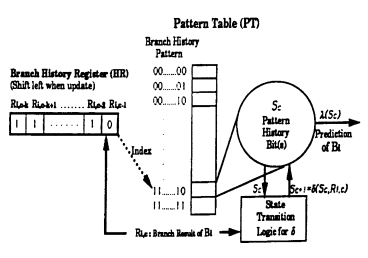
\includegraphics[width=6cm]{two_level}\\
    \footnotesize FIG. 1. Two-Level adaptive prediction
\end{center}

\begin{flushleft}
    \ \ \ \ \ \ 當前此結構有個問題是如果當前有兩個相同\ pattern 因此他們會共用到同個\ saturating counter,\
    但如果這兩個\ pattern 處於完全相反的\ branch 結果, \
    例如一者為經常做\ branch 另一者則經常不做\ branch,\
    將會導致我們這個 branch prediction 失準。\
    因此我使用\ gshare 的方式改動原本\ two-Level adaptive prediction 的架構,\
    原本\ Branch history register 會作為\ Pattern History 的\ index,\
    現在我將\ Branch history register 的值先與\ PC 做一次\ xor 後再作為\ Pattern History 的\ index,\
    以此降低發生\ conflict 的次數。\
    完整的架構圖如\ FIG. 2. 所示。\newline

    \ \ \ \ \ \ 在實做上需要考量的參度為\ Branch history register 的長度,\
    以及需要做\ xor 的\ bit, 例如如果長度為\ 5,\
    可以選擇拿\ PC [5:0] 也可以拿 \ PC [6:1] 下去做運算,\
    唯一可以確定的是不能選擇太過接近\ MSB 的部份做運算避免每個指令過少情況導致大多數分支指令的\ MSB 完全相同,\
    其餘因素只能透過大量測試確認何者為最佳。\
\end{flushleft}

\columnbreak

\begin{center}
    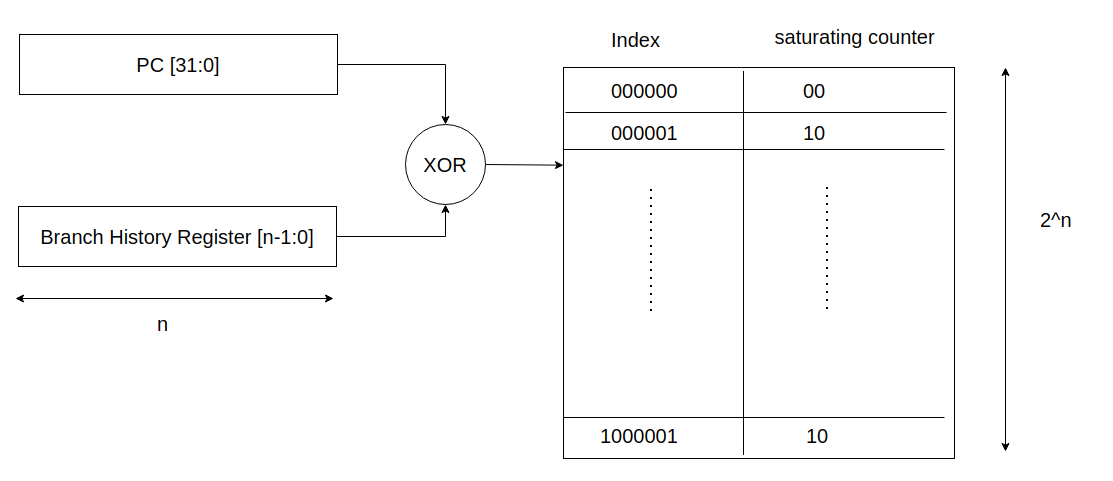
\includegraphics[width=9cm]{two_level_02}\\
    \footnotesize FIG. 2. Two-Level adaptive prediction
\end{center}

\begin{center}
    \section*{IMPLEMENTATION}
\end{center}

\begin{flushleft}
    \ \ \ \ \ \ 首先我先將架構改寫完後用自己改寫的\ Dhrystone 測試確定速度上有提昇後,\
    使用原本的\ Dhrystone 進行測試並且找出最佳的參數且同時驗證\ Dhrystone 上的結果與答案正確。\
    根據\ TABLE. 5. , \ index 表明以\ PC 哪些\ bit 與進行\ Branch History Register xor 運算,\
    同時也嘗試了不同長度的\ Branch History Register, \
    可以看到這些參數與\ DMIPS 可能沒有直接關係,\
    而最佳者\ DMIPS 為\ 0.94859,\
    不確定其餘參數是否可以獲得更佳的\ DMIPS,\
    一切都得經過實際測試才知道。\newline

    \ \ \ \ \ \ 接著我以最佳者的\ DMIPS 以\ ILA 查看分支預測的過程,\
    可以發現與當前\ BHT entry 為\ 64 的差異點是\ miss 次數,\
    在\ BHT entry 為\ 64 時大約每個\ iteration miss 5 次,\
    但在\ two level predictor 中在穩定後約每個\ iteration miss 10 次,\
    我想到可能造成的原因是衝突的問題可能依然沒有解決,\
    仍然有少量的衝突發生造成不同分支指令共用了同個\ saturating counter。\
    不過儘管無法再多改進\ DMIPS,\
    仍然可以使用自己針對\ saturating counter 所設計的程式進行驗證。

\end{flushleft}

\begin{center}
    \begin{tabular}{||c c c c c c ||} 
        \hline
        index & DMIPS & index & DMIPS & index & DMIPS \\ [1.0ex] 
        \hline\hline
        [4:0] & 0.90919 & [5:0] & 0.92999 & [6:0] &  0.92395  \\ 
        \hline
        [5:1] & 0.92395 &  &  &  &  \\ 
        \hline
        [6:2] & 0.92999 & [7:2] & 0.93919 &  &    \\
        \hline
        [7:3] & 0.93919 & [8:3] & 0.91799 & [9:3] & 0.91799  \\
        \hline
        [8:4] & 0.92696 & [9:4] & 0.94859 & [10:4] & 0.94859\\
        \hline
         &    &   [10:5] & 0.94543
    \end{tabular}
\end{center}

\begin{center}
    \footnotesize TABLE. 5. Result of different parameter
\end{center}

\begin{flushleft}
    \ \ \ \ \ \ TABLE 6. 為使用自己改的\ Dhrystone 進行測試的結果,\
    tpye 為 \ D 表示為當前 Aquila 採用並改為\ BHT entry 為\ 64 的版本,\
    tpye 為 \ T 表示已經改寫為\ two level 的版本。\
    \ out 與\ in 分別表示外迴圈與內迴圈次數。\
    根據前面描述改寫的\ Dhrystone,\
    在內迴圈只有單一層的情況,\
    two level 已經跑得比原本\ BHT 為 \ 64 entry 的\ predictor 還快了,\
    如果多增加內迴圈數量或者增加外迴圈次數將可以拉開更多兩者執行時間。\
    因此確認\ two level 在某些情況確實可以處理得比\ Dynamic branch prediction 還好。
\end{flushleft}

\begin{center}
    \begin{tabular}{||c c c c ||} 
        \hline
        type & out & in & time(s)   \\ [1.0ex] 
        \hline\hline
        D & 10000000 & 1 & 6.2  \\ 
        \hline
        T & 10000000 & 1 & 6.6  \\ 
        \hline
        D & 50000000 & 1 & 33.0  \\ 
        \hline
        T & 50000000 & 1 & 29.0  \\ 
        \hline
        D & 10000000 & 2 & 12.8  \\ 
        \hline
        T & 10000000 & 2 & 10.4 \\ 
        \hline
        D & 10000000 & 4 & 25.2  \\ 
        \hline
        T & 10000000 & 4 & 21.6 \\ 
        \hline
    \end{tabular}
\end{center}
\begin{center}
    \footnotesize TABLE. 6. Result of executing my Dhrystone
\end{center}

\newpage

\begin{center}
    \section*{Hit and Miss}
\end{center}

\begin{flushleft}
    \ \ \ \ \ \ 現在已經完成對\ saturating counter 與 \ two-level predictor 的分析,\
    最後附上\ hit 與 \ miss 的兩者結果,\ 
    在這裡的 \ hit 與 \ miss 指的是分支預測成功或是失敗,\
    並非像是在\ cache 中的是否存在於\ BHT entry 中的概念。\
    而因為在進入主要 \ Dhrystone 主要迴圈前無論對任一型態的預測器\ hit 或是\ miss 數量都一樣,\
    次數分別為\ hit: 0x264da 與 \ miss: 0x7b,\
    因此這邊的數據直接以跑完\ Dhrystone 的\ hit 與\ miss 最為最終數值。\

    \begin{center}
        \begin{tabular}{||c c c c c ||} 
            \hline
            type & runs & Hit & Miss & H/M rate \\ [1.0ex] 
            \hline\hline
            32 entry BHT & 10000000 & 0x10674a1 & 0x4c4bf8 & 0.774\\ 
            \hline
            64 entry BHT & 10000000 & 0x32bc57c & 0x4c4bf9 & 0.914\\ 
            \hline
            two-level & 10000000 & 0x2b15676 & 0xc6ba51 & 0.776\\ 
            \hline
        \end{tabular}
    \end{center}
\end{flushleft}
\begin{center}
    \footnotesize TABLE. 7. number of Hit and Miss 
\end{center}

\begin{flushleft}
    \ \ \ \ \ \ 從\ Hit 與\ Miss 數據可以用來再次驗證之前的理論,\
    在\ BHT 從\ 32 entry 上升到\ 64 entry,\
    發生了\ BHT entry 不夠導致每次都需要加進\ BHT 內導致發生初始化進而不做預測,\
    因此透過\ TABLE. 7. 我們可以再次驗證到這個想法的正確性,\
    可以看到\ 32 entry 與\ 64 entry 的\ miss 次數甚至幾乎相同,\
    而\ 32 entry 真的也少猜了很多次,\ 64 entry 反之因為不會有初始化問題,\
    導致獲得很大的提昇。\
    而\ two level predictor 贏過 \ 32 entry 的原因也幾乎與上述相同,\
    主要是不發生初始化可以有較多預測機會,\
    所以最後獲得較多的\ hit 次數。\
    雖然\ miss 次數也因此較多但也如同我們前面所述的\ miss 次數其實不影響,\
    最差情況也只會變回跟不猜測的狀態一樣。\
\end{flushleft}

\begin{flushleft}
    \ \ \ \ \ \ 在做紀錄\ hit 與\ miss 次數的時候一開始遇到數值一直不穩定的情況,\
    一開始我以為是發生\ overflow 的情況,\
    改了好幾次甚至存到\ 100 bit 的大小還是沒有解決,\
    降低\ Dhrystone 內的主迴圈次數也還是沒有解決,\
    後來發現應該是\ uart 的問題,\
    只要用\ pc 去針對是否為非\ Dhrystone 內容加以判斷後就解決了,\
    前前後後又多花上不少時間QQ。
\end{flushleft}

\begin{center}
    \section*{SUMMARY}
\end{center}

\begin{flushleft}
    \ \ \ \ \ \ 此篇報告我們先分析了當前\ Aquila 的分支預測情形,\
    並且對\ BHT size 做變動,\
    在\ BHT entry 為 \ 64 時我們得到了\ 0.97457,\
    透過分析知道了\ Dhrystone 內的迴圈共有\ 36 個分支指令,\
    同時也因此知道將\ BHT entry 從 \ 32 拉到 \ 64 時會有顯著提昇的原因。\
    接著說明當前\ Aquila 採用的\ Dynamic branch prediction 可能無法解決的情形,\
    並將其以組合語言實現用來測試\ two level adaptive predictor 可以適應這個情況。\
    接著探討在此次作業內的 two level adaptive predictor 的架構,\
    並且為了避免\ pattern 發生衝突進行改動,\
    接著將\ Dhrystone stone 執行在\ two level adaptive predictor 上,\
    驗證結果正確且得到最佳的結果為 \ 0.94859。\
    最後以我自己改寫的\ Dhrystone 進行\ two level adaptive predictor 與當前\ Aquila 的\ branch prediction 進行的比較,\
    驗證的確\ two level adaptive predictor 克服了缺點且跑得比較快。\newline

    \ \ \ \ \ \ 因為版面還有空間想寫些心得,\
    一開始直接使用\ ILA 想觀察\ BHT entry 數量是否會影響 \ DMIPS,\
    後來才發覺要先用模擬確認都沒問題再上板子會節省相當多時間,\
    直接上板子如果不小心沒寫好就是浪費十分鐘的時間。
    一開始發現\ BHT entry 數量不影響後,\
    老師上課卻提到會有影響,\
    回頭重新看程式碼才發現自己沒有改成功,\
    果然會有重大改變!\
    也因此可以更深入理解其影響因素為何,\
    在計算機組織時其實對分支預測概念模模糊糊,\
    這次作業雖然用了很多時間(期中考大爆炸QQ)可是同時也對分支預測的印象更深了不少!\
\end{flushleft}

\columnbreak

\ 

\end{multicols}


\end{CJK*}
\end{document}